\section{Gaussian process surrogate}

The most popular surrogate model is the Gaussian process, we will now understand model
in more detail. 

\subsection{Exact predictive distribution}
We now show how the preditive distribution is calculated exact for
Gaussian Processes, i.e. 
\begin{equation}\label{GP_predictive}
    p(y|x,\mathcal{D}) = \int \mathcal{N}(y|f(x), \sigma^2) p(f(x)|\mathcal{D})df(x)
\end{equation}
we will soon see that $p(f(x)|\mathcal{D}) = \mathcal{N}(f(x)| .., ...)$ and
and thereby that we have a marginal Gaussian distribution for $f(x)$ and a 
conditional Gaussian distribution of $y$ given $f(x)$, giving us the marginalized
distribtuion, $p(y|x,\mathcal{D})$, using formulars \eqref{marginal_distribution}. 

\begin{testexample2}[Trick with normal distributions [from Bishops book?]]
    Given a marginal Gaussian distribution of $x$ and a conditional Gaussian distribution
    of $y$ given $x$ of the form, 
    \begin{align*}
        p(x) &= \mathcal{N}(x|\mu, \Lambda^{-1})\\
        p(y|x) &= \mathcal{N}(x|Ax+b, L^{-1})
    \end{align*}
    then the marginal distribution of $y$ and the conditional distribution of $x$ given $y$
    have the form, 
    \begin{align}
        p(y) &= \mathcal{N}(y|A\mu+b,L^{-1}+A \Lambda^{-1}A^T) \label{marginal_distribution}\\
        p(x|y) &= \mathcal{N}(x|\Gamma \mu+\Gamma [A^TL(y-b)],\Gamma )\\
        \Gamma &:= (\Lambda +A^TLA)^{-1}
    \end{align}
\end{testexample2}

\subsubsection*{Posterior function}
Recall we assume $\textbf{f} = (f(\textbf{x}_1), \dots, f(\textbf{x}_n))$ is the parameters in 
our model, therefore we call $p(\textbf{f}|\mathcal{D})$ the posterior distribution. However, 
what is of real interest is the function values on unobserved locations, thereby we 
extend $\textbf{f}$ to be a function, i.e. an infinitely dimentional vector. We call this 
quantaty \textit{the posterior function} 
\begin{equation}\label{posterior_function}
    p(f(\cdot)|\mathcal{D})= \int p(f(\cdot)|\textbf{x}, \textbf{f})p(\textbf{f}|\mathcal{D})d\textbf{f}.
\end{equation}
% The connection between the two posteriors is given here:
% $$p(f(\cdot)|\mathcal{D}) = \int p(f(\cdot)|\textbf{x}, \textbf{f})p(\textbf{f}|\mathcal{D})d\textbf{f}$$
Prior we assume that the function takes values accoring to
$$p(\textbf{f}|\textbf{x}) = \mathcal{N}(\textbf{f}|\textbf{0}, c(\textbf{x}, \textbf{x}))$$ where
the covariance is defined at kernel evaluation for each pair of $\textbf{x}$, where $c(\cdot,
\cdot)$ is a covariance function, chosen to be the Matérn covariance function,

  $$c(\textbf{x}, \textbf{x}) = \begin{bmatrix}
    c(x_1,x_1) & \dots & c(x_1,x_n)\\
    \vdots& \ddots\\
    c(x_n,x_1) & \dots & c(x_n,x_n)
\end{bmatrix}\hspace{1cm} c(x, y) := Matern(x,y)...$$ 

\begin{figure}[h]
    \centering
    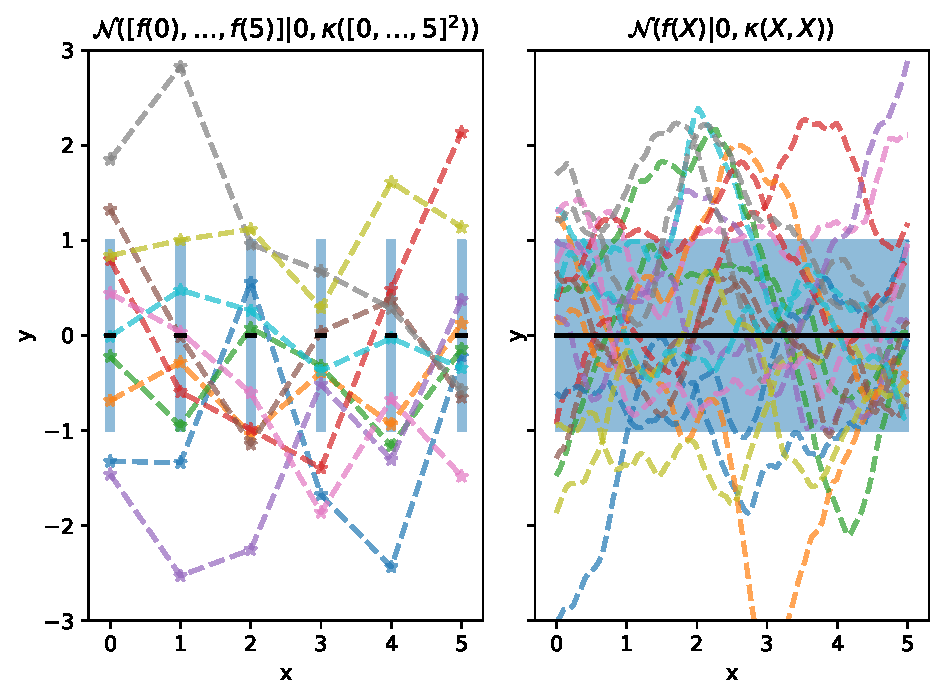
\includegraphics[width = \textwidth]{Pictures/GP_samples_mattern.pdf}
    \caption{Realisations> Illustartaion of GP is just samples from a multivariate normal distribution. In the
    limit the we have a infinite-variate normal distribution, which we call a GP.}
\end{figure}

Appendix <...> tries to give the intuition why this makes sense. 

We now calculate the first term in the integral \eqref{posterior_function}, 
$p(f(\cdot)|\textbf{x}, \textbf{f})$ using that we have the joint prior 
distribution, 
\begin{align}
    p(f(\cdot),\textbf{f}|\textbf{x}) = \mathcal{N}\left(\begin{bmatrix}
        f(\cdot)\\ \textbf{f}
    \end{bmatrix} \middle| \begin{bmatrix}
        0\\ \textbf{0}
    \end{bmatrix}, \begin{bmatrix}
        c(\cdot, \cdot) & c(\cdot,\textbf{x})\\
        c(\textbf{x}, \cdot) & c(\textbf{x}, \textbf{x})
    \end{bmatrix} \right)
\end{align}

And the conditonal of a joint Gaussian is given using <ref> 
$$p(f(\cdot)|\textbf{x}, \textbf{f}) = \mathcal{N}(f(\cdot)|c(\cdot, \cdot)^{-1}c(\cdot, \textbf{x})\textbf{f}, c(\cdot, \cdot)^{-1})$$

Next we calculate the last term in the integral \eqref{posterior_function}, 
$p(\textbf{f}|\mathcal{D})$, i.e. the posterior distribution. Assuming iid data, 
i.e. $p(y_1,\dots, y_n|x_1,\dots, x_n, \textbf{f}) = \prod_{i=1}^n p(y_i|x_i,\textbf{f}_i)$
and that the likelihood is Gaussian with mean $\textbf{f}$ and variance $\sigma^2 I_n$. 

\begin{align*}
    p(\textbf{f}|\mathcal{D}) &\propto p(\textbf{f}|x)\prod_{i=1}^n p(y_i|x_i,\textbf{f}_i)\\
    &= \mathcal{N}(\textbf{f}|\textbf{0},c(\textbf{x}, \textbf{x})) \prod_{i=1}^n \mathcal{N}(y|\textbf{f}_i,\sigma^2)\\
    &= \mathcal{N}(\textbf{f}|\textbf{0}, c(\textbf{x}, \textbf{x})) \mathcal{N}(\textbf{y}|\textbf{f},\sigma^2 I_n)
\end{align*}
now from <ref> we have that the posterior is the following Gaussian: 
\begin{equation*}
    p(\textbf{f}|\mathcal{D}) = \mathcal{N}(\textbf{f}|M^{-1} \sigma^{-2}\textbf{y}, M^{-1}) \hspace{0.5cm}M := c(\textbf{x}, \textbf{x})^{-1}+\sigma^{-2} I_n
\end{equation*}
Now we found that both term in the integral \eqref{posterior_function}, and they
are related such that it is possible to use \eqref{marginal_distribution} for arriving 
at (we define $A :=  c(\cdot, \cdot)^{-1} c(\cdot, \textbf{x})$), 
$$p(f(\cdot)|\mathcal{D}) = \mathcal{N}(f(\cdot)|AM^{-1}\sigma^{-2}\textbf{y}, c(\cdot, \cdot)^{-1}+
AM^{-1}A^T)$$

Finally we found that both terms in the integral \eqref{GP_predictive} also is related
in a simlar way, and we use \eqref{marginal_distribution}, again to arrive at the predictive
distribtuion, 
$$p(y_*|x_*,\mathcal{D}) = \mathcal{N}(y_*|AM^{-1}\sigma^{-2}\textbf{y}, c(x_*, x_*)^{-1}+
AM^{-1}A^T+\sigma^2)$$

\todo{Some questions about a naive approach..!}

\subsubsection*{Learning - Emperical bayes inference}

Anther inference which is done is then optimizing the hyper parameters using emperical bayes i.e.
the variance and length scale for the kernel. Here we optimize the marginalized likelihood function
$$p(y_1, \dots, y_n|x_1, \dots, x_n, \theta) = -\frac{1}{2}[(y-\mu)^T (\Sigma+N)^{-1}(y-\mu)+ \log |\Sigma+N|+n \log 2\pi]$$
<and how to get to there?>

\todo{Model assessment becomes trivial in light of the model posterior if we
simply establish preferences over models according to their posterior
probability. When using the uniform model prior (4.6)
 the model posterior is proportional to the marginal likelihood alone,
which can be then used directly for model assessment. ??! Youtube - good video! Go through that!}

